\documentclass{article}
\usepackage{geometry}
\usepackage{pgf-umlcd}
\usepgflibrary{arrows}
\geometry{a2paper, scale = 0.95}
\pagestyle{empty}
\title{ComputerProgramDesign}
\author{Xuc Pan}
\date{July 2023}

\begin{document}

\centering

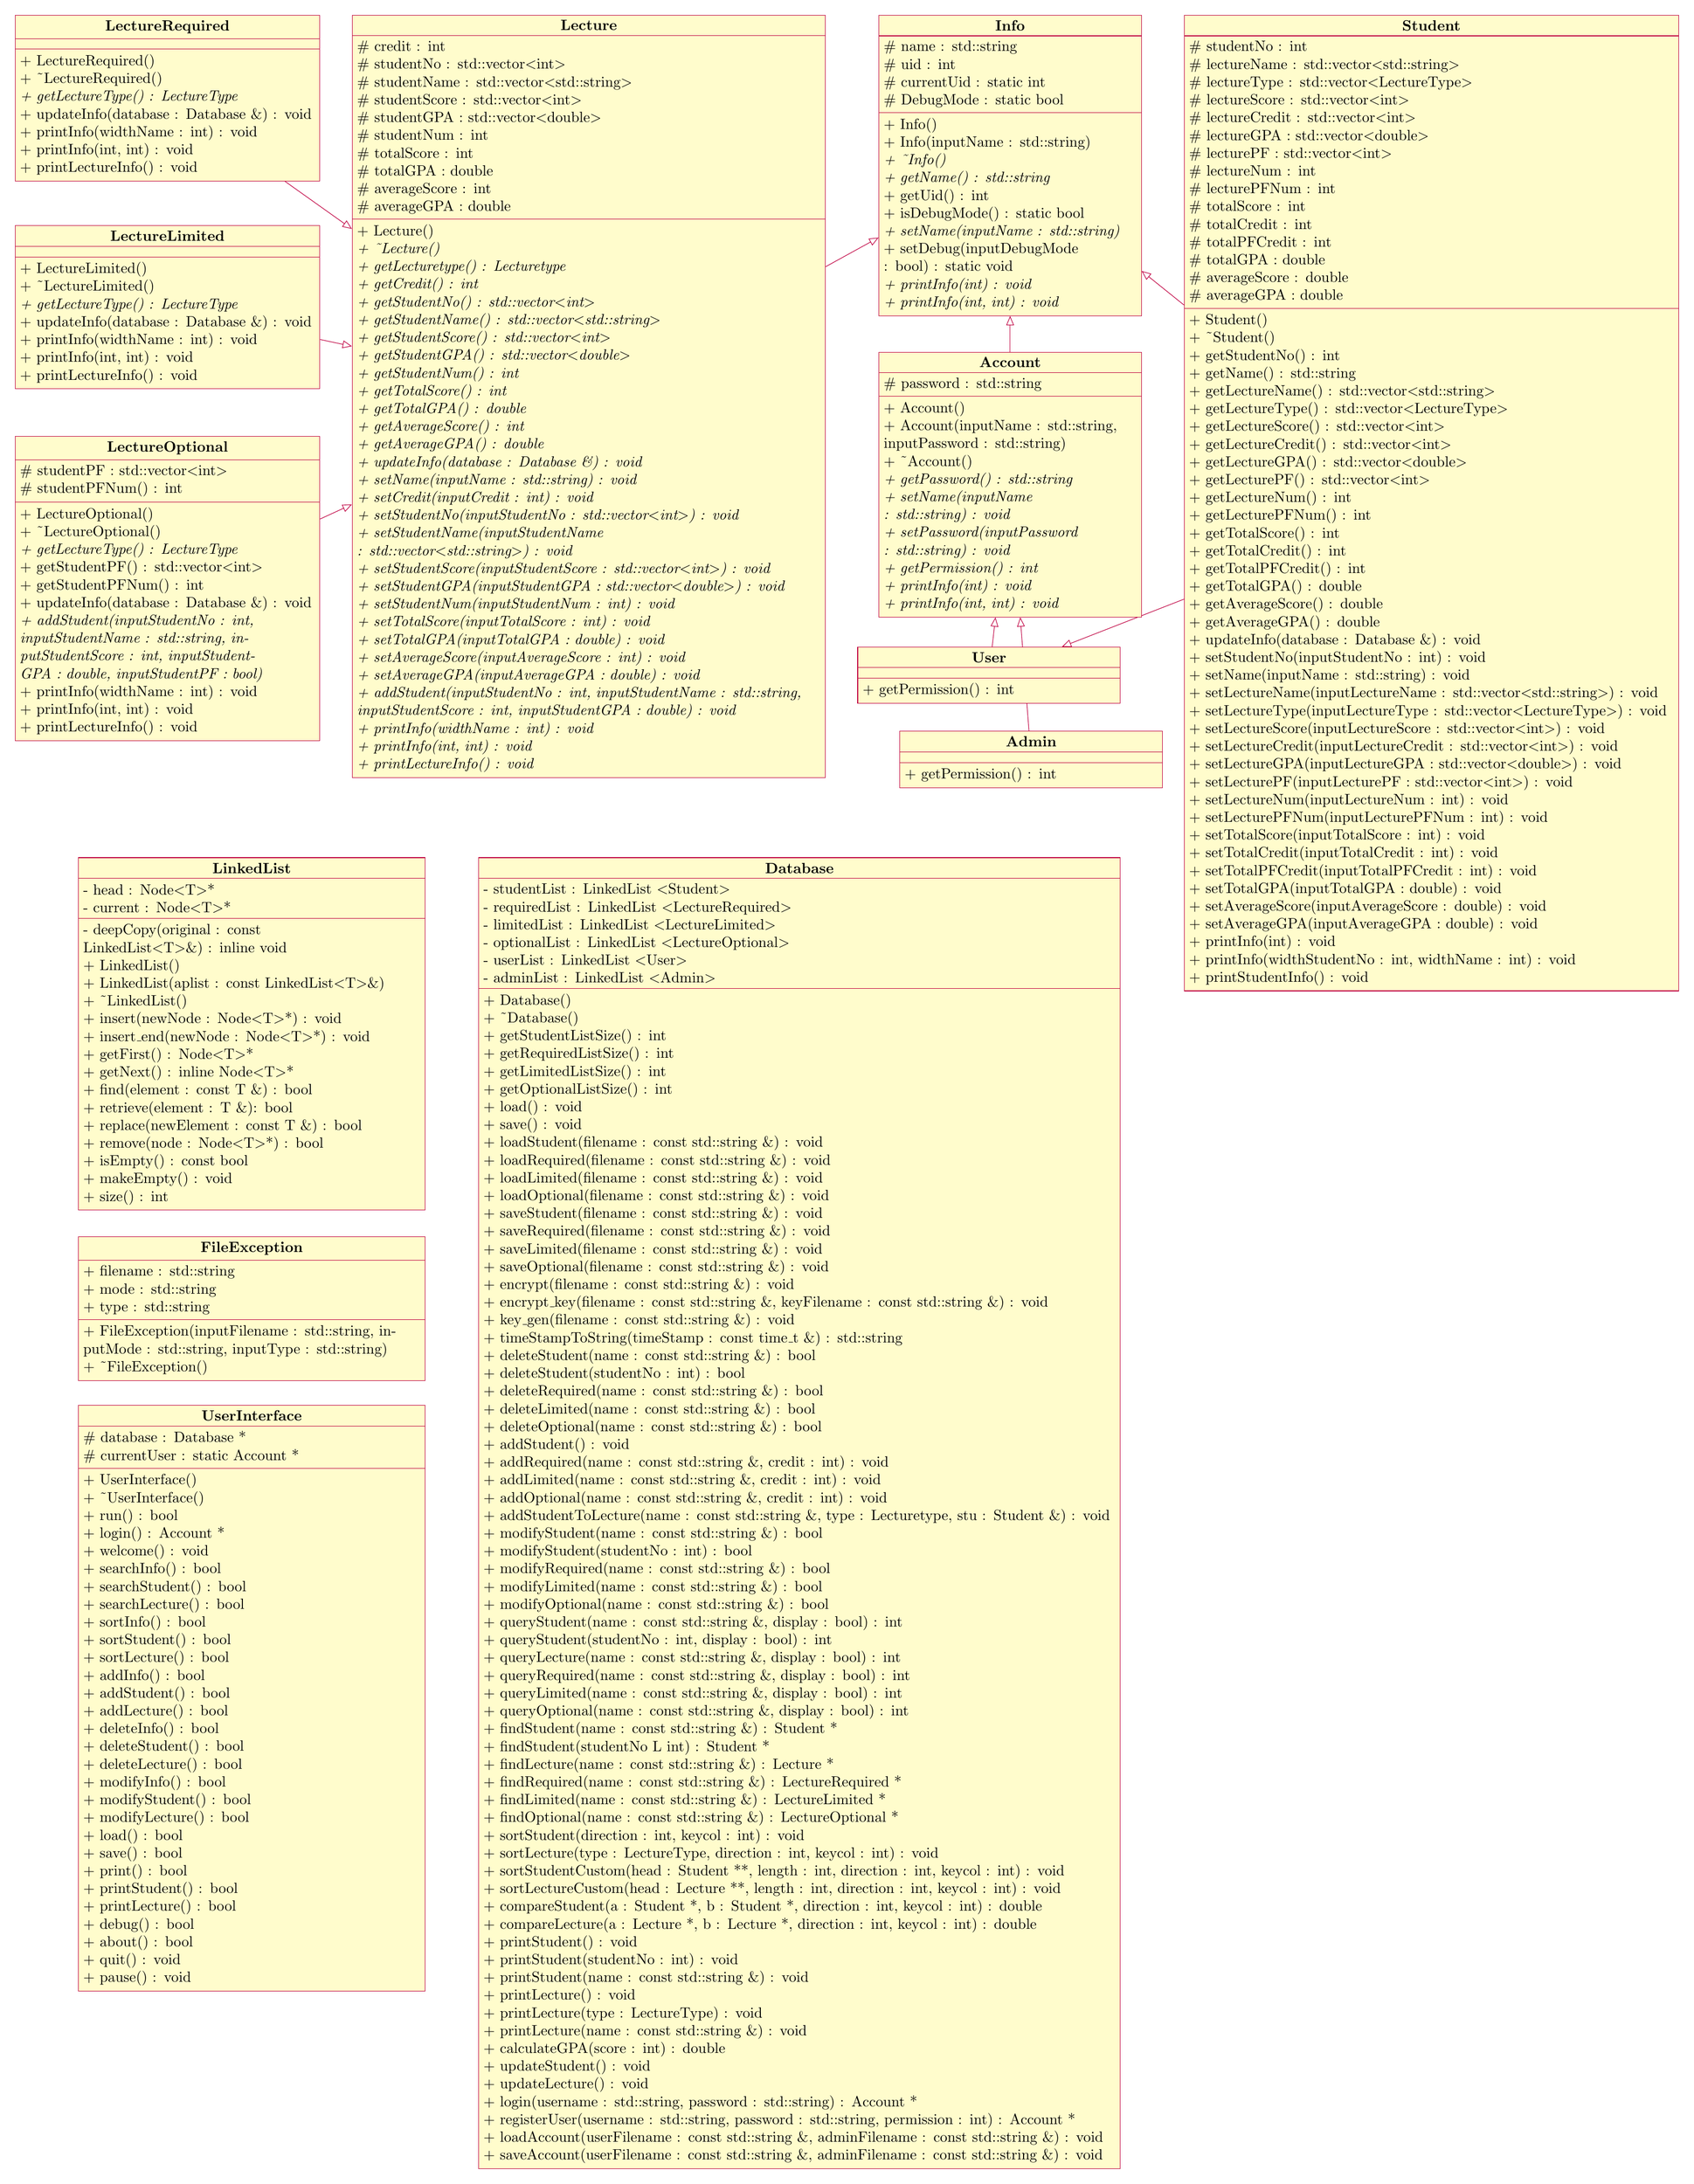
\begin{tikzpicture}

 \begin{class}[text width=6cm]{Info}{0,0}
  \attribute{\# name : std::string}
  \attribute{\# uid : int}
  \attribute{\# currentUid : static int}
  \attribute{\# DebugMode : static bool}
  \operation{+ Info()}
  \operation{+ Info(inputName : std::string)}
  \operation[0]{+ \textasciitilde Info()}
  \operation[0]{+ getName() : std::string}
  \operation{+ getUid() : int}
  \operation{+ isDebugMode() : static bool}
  \operation[0]{+ setName(inputName : std::string)}
  \operation{+ setDebug(inputDebugMode : bool) : static void}
  \operation[0]{+ printInfo(int) : void}
  \operation[0]{+ printInfo(int, int) : void}
 \end{class}

 \begin{class}[text width=6cm]{Account}{0,-8}
 \inherit{Info}
  \attribute{\# password : std::string}
  \operation{+ Account()}
  \operation{+ Account(inputName : std::string, inputPassword : std::string)}
  \operation{+ \textasciitilde Account()}
  \operation[0]{+ getPassword() : std::string}
  \operation[0]{+ setName(inputName : std::string) : void}
  \operation[0]{+ setPassword(inputPassword : std::string) : void}
  \operation[0]{+ getPermission() : int}
  \operation[0]{+ printInfo(int) : void}
  \operation[0]{+ printInfo(int, int) : void}
 \end{class}

 \begin{class}[text width=6cm]{User}{-0.5,-15}
  \inherit{Account}
  \operation{+ getPermission() : int}
 \end{class}

 \begin{class}[text width=6cm]{Admin}{0.5,-17}
  \inherit{Account}
  \operation{+ getPermission() : int}
 \end{class}

 \begin{class}[text width=11.5cm]{Student}{10,0}
  \inherit{Info}
  \inherit{User}
  \attribute{\# studentNo : int}
  \attribute{\# lectureName : std::vector\textless std::string\textgreater}
  \attribute{\# lectureType : std::vector\textless LectureType\textgreater}
  \attribute{\# lectureScore : std::vector\textless int\textgreater}
  \attribute{\# lectureCredit : std::vector\textless int\textgreater}
  \attribute{\# lectureGPA : std::vector\textless double\textgreater}
  \attribute{\# lecturePF : std::vector\textless int\textgreater}
  \attribute{\# lectureNum : int}
  \attribute{\# lecturePFNum : int}
  \attribute{\# totalScore : int}
  \attribute{\# totalCredit : int}
  \attribute{\# totalPFCredit : int}
  \attribute{\# totalGPA : double}
  \attribute{\# averageScore : double}
  \attribute{\# averageGPA : double}
  \operation{+ Student()}
  \operation{+ \textasciitilde Student()}
  \operation{+ getStudentNo() : int}
  \operation{+ getName() : std::string}
  \operation{+ getLectureName() : std::vector\textless std::string\textgreater}
  \operation{+ getLectureType() : std::vector\textless LectureType\textgreater}
  \operation{+ getLectureScore() : std::vector\textless int\textgreater}
  \operation{+ getLectureCredit() : std::vector\textless int\textgreater}
  \operation{+ getLectureGPA() : std::vector\textless double\textgreater}
  \operation{+ getLecturePF() : std::vector\textless int\textgreater}
  \operation{+ getLectureNum() : int}
  \operation{+ getLecturePFNum() : int}
  \operation{+ getTotalScore() : int}
  \operation{+ getTotalCredit() : int}
  \operation{+ getTotalPFCredit() : int}
  \operation{+ getTotalGPA() : double}
  \operation{+ getAverageScore() : double}
  \operation{+ getAverageGPA() : double}
  \operation{+ updateInfo(database : Database \&) : void}
  \operation{+ setStudentNo(inputStudentNo : int) : void}
  \operation{+ setName(inputName : std::string) : void}
  \operation{+ setLectureName(inputLectureName : std::vector\textless std::string\textgreater) : void}
  \operation{+ setLectureType(inputLectureType : std::vector\textless LectureType\textgreater) : void}
  \operation{+ setLectureScore(inputLectureScore : std::vector\textless int\textgreater) : void}
  \operation{+ setLectureCredit(inputLectureCredit : std::vector\textless int\textgreater) : void}
  \operation{+ setLectureGPA(inputLectureGPA : std::vector\textless double\textgreater) : void}
  \operation{+ setLecturePF(inputLecturePF : std::vector\textless int\textgreater) : void}
  \operation{+ setLectureNum(inputLectureNum : int) : void}
  \operation{+ setLecturePFNum(inputLecturePFNum : int) : void}
  \operation{+ setTotalScore(inputTotalScore : int) : void}
  \operation{+ setTotalCredit(inputTotalCredit : int) : void}
  \operation{+ setTotalPFCredit(inputTotalPFCredit : int) : void}
  \operation{+ setTotalGPA(inputTotalGPA : double) : void}
  \operation{+ setAverageScore(inputAverageScore : double) : void}
  \operation{+ setAverageGPA(inputAverageGPA : double) : void}
  \operation{+ printInfo(int) : void}
  \operation{+ printInfo(widthStudentNo : int, widthName : int) : void}
  \operation{+ printStudentInfo() : void}
 \end{class}

 \begin{class}[text width = 11cm]{Lecture}{-10,0}
  \inherit{Info}
  \attribute{\# credit : int}
  \attribute{\# studentNo : std::vector\textless int\textgreater}
  \attribute{\# studentName : std::vector\textless std::string\textgreater}
  \attribute{\# studentScore : std::vector\textless int\textgreater}
  \attribute{\# studentGPA : std::vector\textless double\textgreater}
  \attribute{\# studentNum : int}
  \attribute{\# totalScore : int}
  \attribute{\# totalGPA : double}
  \attribute{\# averageScore : int}
  \attribute{\# averageGPA : double}
  \operation{+ Lecture()}
  \operation[0]{+ \textasciitilde Lecture()}
  \operation[0]{+ getLecturetype() : Lecturetype}
  \operation[0]{+ getCredit() : int}
  \operation[0]{+ getStudentNo() : std::vector\textless int\textgreater}
  \operation[0]{+ getStudentName() : std::vector\textless std::string\textgreater}
  \operation[0]{+ getStudentScore() : std::vector\textless int\textgreater}
  \operation[0]{+ getStudentGPA() : std::vector\textless double\textgreater}
  \operation[0]{+ getStudentNum() : int}
  \operation[0]{+ getTotalScore() : int}
  \operation[0]{+ getTotalGPA() : double}
  \operation[0]{+ getAverageScore() : int}
  \operation[0]{+ getAverageGPA() : double}
  \operation[0]{+ updateInfo(database : Database \&) : void}
  \operation[0]{+ setName(inputName : std::string) : void}
  \operation[0]{+ setCredit(inputCredit : int) : void}
  \operation[0]{+ setStudentNo(inputStudentNo : std::vector\textless int\textgreater) : void}
  \operation[0]{+ setStudentName(inputStudentName : std::vector\textless std::string\textgreater) : void}
  \operation[0]{+ setStudentScore(inputStudentScore : std::vector\textless int\textgreater) : void}
  \operation[0]{+ setStudentGPA(inputStudentGPA : std::vector\textless double\textgreater) : void}
  \operation[0]{+ setStudentNum(inputStudentNum : int) : void}
  \operation[0]{+ setTotalScore(inputTotalScore : int) : void}
  \operation[0]{+ setTotalGPA(inputTotalGPA : double) : void}
  \operation[0]{+ setAverageScore(inputAverageScore : int) : void}
  \operation[0]{+ setAverageGPA(inputAverageGPA : double) : void}
  \operation[0]{+ addStudent(inputStudentNo : int, inputStudentName : std::string, inputStudentScore : int, inputStudentGPA : double) : void}
  \operation[0]{+ printInfo(widthName : int) : void}
  \operation[0]{+ printInfo(int, int) {}: void}
  \operation[0]{+ printLectureInfo() : void}
 \end{class}

 \begin{class}[text width = 7cm]{LectureRequired}{-20,0}
  \inherit{Lecture}
  \operation{+ LectureRequired()}
  \operation{+ \textasciitilde LectureRequired()}
  \operation[0]{+ getLectureType() : LectureType}
  \operation{+ updateInfo(database : Database \&) : void}
  \operation{+ printInfo(widthName : int) : void}
  \operation{+ printInfo(int, int) : void}
  \operation{+ printLectureInfo() : void}
 \end{class}

 \begin{class}[text width = 7cm]{LectureLimited}{-20,-5}
  \inherit{Lecture}
  \operation{+ LectureLimited()}
  \operation{+ \textasciitilde LectureLimited()}
  \operation[0]{+ getLectureType() : LectureType}
  \operation{+ updateInfo(database : Database \&) : void}
  \operation{+ printInfo(widthName : int) : void}
  \operation{+ printInfo(int, int) : void}
  \operation{+ printLectureInfo() : void}
 \end{class}

 \begin{class}[text width = 7cm]{LectureOptional}{-20,-10}
  \inherit{Lecture}
  \attribute{\# studentPF : std::vector\textless int\textgreater}
  \attribute{\# studentPFNum() : int}
  \operation{+ LectureOptional()}
  \operation{+ \textasciitilde LectureOptional()}
  \operation[0]{+ getLectureType() : LectureType}
  \operation{+ getStudentPF() : std::vector\textless int\textgreater}
  \operation{+ getStudentPFNum() : int}
  \operation{+ updateInfo(database : Database \&) : void}
  \operation[0]{+ addStudent(inputStudentNo : int, inputStudentName : std::string, inputStudentScore : int, inputStudentGPA : double, inputStudentPF : bool)}
  \operation{+ printInfo(widthName : int) : void}
  \operation{+ printInfo(int, int) : void}
  \operation{+ printLectureInfo() : void}
 \end{class}

 \begin{class}[text width = 8cm]{LinkedList}{-18, -20}
  \attribute{- head : Node\textless T\textgreater *}
  \attribute{- current : Node\textless T\textgreater *}
  \operation{- deepCopy(original : const LinkedList\textless T\textgreater \&) : inline void}
  \operation{+ LinkedList()}
  \operation{+ LinkedList(aplist : const LinkedList\textless T\textgreater \&)}
  \operation{+ \textasciitilde LinkedList()}
  \operation{+ insert(newNode : Node\textless T\textgreater *) : void}
  \operation{+ insert\_end(newNode : Node\textless T\textgreater *) : void}
  \operation{+ getFirst() : Node\textless T\textgreater *}
  \operation{+ getNext() : inline Node\textless T\textgreater *}
  \operation{+ find(element : const T \&) : bool}
  \operation{+ retrieve(element : T \&): bool}
  \operation{+ replace(newElement : const T \&) : bool}
  \operation{+ remove(node : Node\textless T\textgreater *) : bool}
  \operation{+ isEmpty() : const bool}
  \operation{+ makeEmpty() : void}
  \operation{+ size() : int}
 \end{class}

 \begin{class}[text width = 8cm]{FileException}{-18, -29}
  \attribute{+ filename : std::string}
  \attribute{+ mode : std::string}
  \attribute{+ type : std::string}
  \operation{+ FileException(inputFilename : std::string, inputMode : std::string, inputType : std::string)}
  \operation{+ \textasciitilde FileException()}
 \end{class}

 \begin{class}[text width = 15cm]{Database}{-5,-20}
  \attribute{- studentList : LinkedList \textless Student\textgreater}
  \attribute{- requiredList : LinkedList \textless LectureRequired\textgreater}
  \attribute{- limitedList : LinkedList \textless LectureLimited\textgreater}
  \attribute{- optionalList : LinkedList \textless LectureOptional\textgreater}
  \attribute{- userList : LinkedList \textless User\textgreater}
  \attribute{- adminList : LinkedList \textless Admin\textgreater}
  \operation{+ Database()}
  \operation{+ \textasciitilde Database()}
  \operation{+ getStudentListSize() : int}
  \operation{+ getRequiredListSize() : int}
  \operation{+ getLimitedListSize() : int}
  \operation{+ getOptionalListSize() : int}
  \operation{+ load() : void}
  \operation{+ save() : void}
  \operation{+ loadStudent(filename : const std::string \&) : void}
  \operation{+ loadRequired(filename : const std::string \&) : void}
  \operation{+ loadLimited(filename : const std::string \&) : void}
  \operation{+ loadOptional(filename : const std::string \&) : void}
  \operation{+ saveStudent(filename : const std::string \&) : void}
  \operation{+ saveRequired(filename : const std::string \&) : void}
  \operation{+ saveLimited(filename : const std::string \&) : void}
  \operation{+ saveOptional(filename : const std::string \&) : void}
  \operation{+ encrypt(filename : const std::string \&) : void}
  \operation{+ encrypt\_key(filename : const std::string \&, keyFilename : const std::string \&) : void}
  \operation{+ key\_gen(filename : const std::string \&) : void}
  \operation{+ timeStampToString(timeStamp : const time\_t \&) : std::string}
  \operation{+ deleteStudent(name : const std::string \&) : bool}
  \operation{+ deleteStudent(studentNo : int) : bool}
  \operation{+ deleteRequired(name : const std::string \&) : bool}
  \operation{+ deleteLimited(name : const std::string \&) : bool}
  \operation{+ deleteOptional(name : const std::string \&) : bool}
  \operation{+ addStudent() : void}
  \operation{+ addRequired(name : const std::string \&, credit : int) : void}
  \operation{+ addLimited(name : const std::string \&, credit : int) : void}
  \operation{+ addOptional(name : const std::string \&, credit : int) : void}
  \operation{+ addStudentToLecture(name : const std::string \&, type : Lecturetype, stu : Student \&) : void}
  \operation{+ modifyStudent(name : const std::string \&) : bool}
  \operation{+ modifyStudent(studentNo : int) : bool}
  \operation{+ modifyRequired(name : const std::string \&) : bool}
  \operation{+ modifyLimited(name : const std::string \&) : bool}
  \operation{+ modifyOptional(name : const std::string \&) : bool}
  \operation{+ queryStudent(name : const std::string \&, display : bool) : int}
  \operation{+ queryStudent(studentNo : int, display : bool) : int}
  \operation{+ queryLecture(name : const std::string \&, display : bool) : int}
  \operation{+ queryRequired(name : const std::string \&, display : bool) : int}
  \operation{+ queryLimited(name : const std::string \&, display : bool) : int}
  \operation{+ queryOptional(name : const std::string \&, display : bool) : int}
  \operation{+ findStudent(name : const std::string \&) : Student *}
  \operation{+ findStudent(studentNo L int) : Student *}
  \operation{+ findLecture(name : const std::string \&) : Lecture *}
  \operation{+ findRequired(name : const std::string \&) : LectureRequired *}
  \operation{+ findLimited(name : const std::string \&) : LectureLimited *}
  \operation{+ findOptional(name : const std::string \&) : LectureOptional *}
  \operation{+ sortStudent(direction : int, keycol : int) : void}
  \operation{+ sortLecture(type : LectureType, direction : int, keycol : int) : void}
  \operation{+ sortStudentCustom(head : Student **, length : int, direction : int, keycol : int) : void}
  \operation{+ sortLectureCustom(head : Lecture **, length : int, direction : int, keycol : int) : void}
  \operation{+ compareStudent(a : Student *, b : Student *, direction : int, keycol : int) : double}
  \operation{+ compareLecture(a : Lecture *, b : Lecture *, direction : int, keycol : int) : double}
  \operation{+ printStudent() : void}
  \operation{+ printStudent(studentNo : int) : void}
  \operation{+ printStudent(name : const std::string \&) : void}
  \operation{+ printLecture() : void}
  \operation{+ printLecture(type : LectureType) : void}
  \operation{+ printLecture(name : const std::string \&) : void}
  \operation{+ calculateGPA(score : int) : double}
  \operation{+ updateStudent() : void}
  \operation{+ updateLecture() : void}
  \operation{+ login(username : std::string, password : std::string) : Account *}
  \operation{+ registerUser(username : std::string, password : std::string, permission : int) : Account *}
  \operation{+ loadAccount(userFilename : const std::string \&, adminFilename : const std::string \&) : void}
  \operation{+ saveAccount(userFilename : const std::string \&, adminFilename : const std::string \&) : void}
 \end{class}

 \begin{class}[text width = 8cm]{UserInterface}{-18, -33}
  \attribute{\# database : Database *}
  \attribute{\# currentUser : static Account *}
  \operation{+ UserInterface()}
  \operation{+ \textasciitilde UserInterface()}
  \operation{+ run() : bool}
  \operation{+ login() : Account *}
  \operation{+ welcome() : void}
  \operation{+ searchInfo() : bool}
  \operation{+ searchStudent() : bool}
  \operation{+ searchLecture() : bool}
  \operation{+ sortInfo() : bool}
  \operation{+ sortStudent() : bool}
  \operation{+ sortLecture() : bool}
  \operation{+ addInfo() : bool}
  \operation{+ addStudent() : bool}
  \operation{+ addLecture() : bool}
  \operation{+ deleteInfo() : bool}
  \operation{+ deleteStudent() : bool}
  \operation{+ deleteLecture() : bool}
  \operation{+ modifyInfo() : bool}
  \operation{+ modifyStudent() : bool}
  \operation{+ modifyLecture() : bool}
  \operation{+ load() : bool}
  \operation{+ save() : bool}
  \operation{+ print() : bool}
  \operation{+ printStudent() : bool}
  \operation{+ printLecture() : bool}
  \operation{+ debug() : bool}
  \operation{+ about() : bool}
  \operation{+ quit() : void}
  \operation{+ pause() : void}
 \end{class}

\end{tikzpicture}

\end{document}
